\section*{Metodolog\'ia}

\subsection*{1. Materiales}
\begin{itemize}
	\item Péndulo de Pohl PHYWE 11214-00
	\item Sensor-CASSY 2
	\item Fuente de poder PHYWE \qty{230}{\volt}
	\item Multímetro digital
	\item Polea, anillo y cuerda ligera
	\item Computador
\end{itemize}

\subsection*{2. Esquema del Montaje}
\begin{figure}[H]
	\centering
	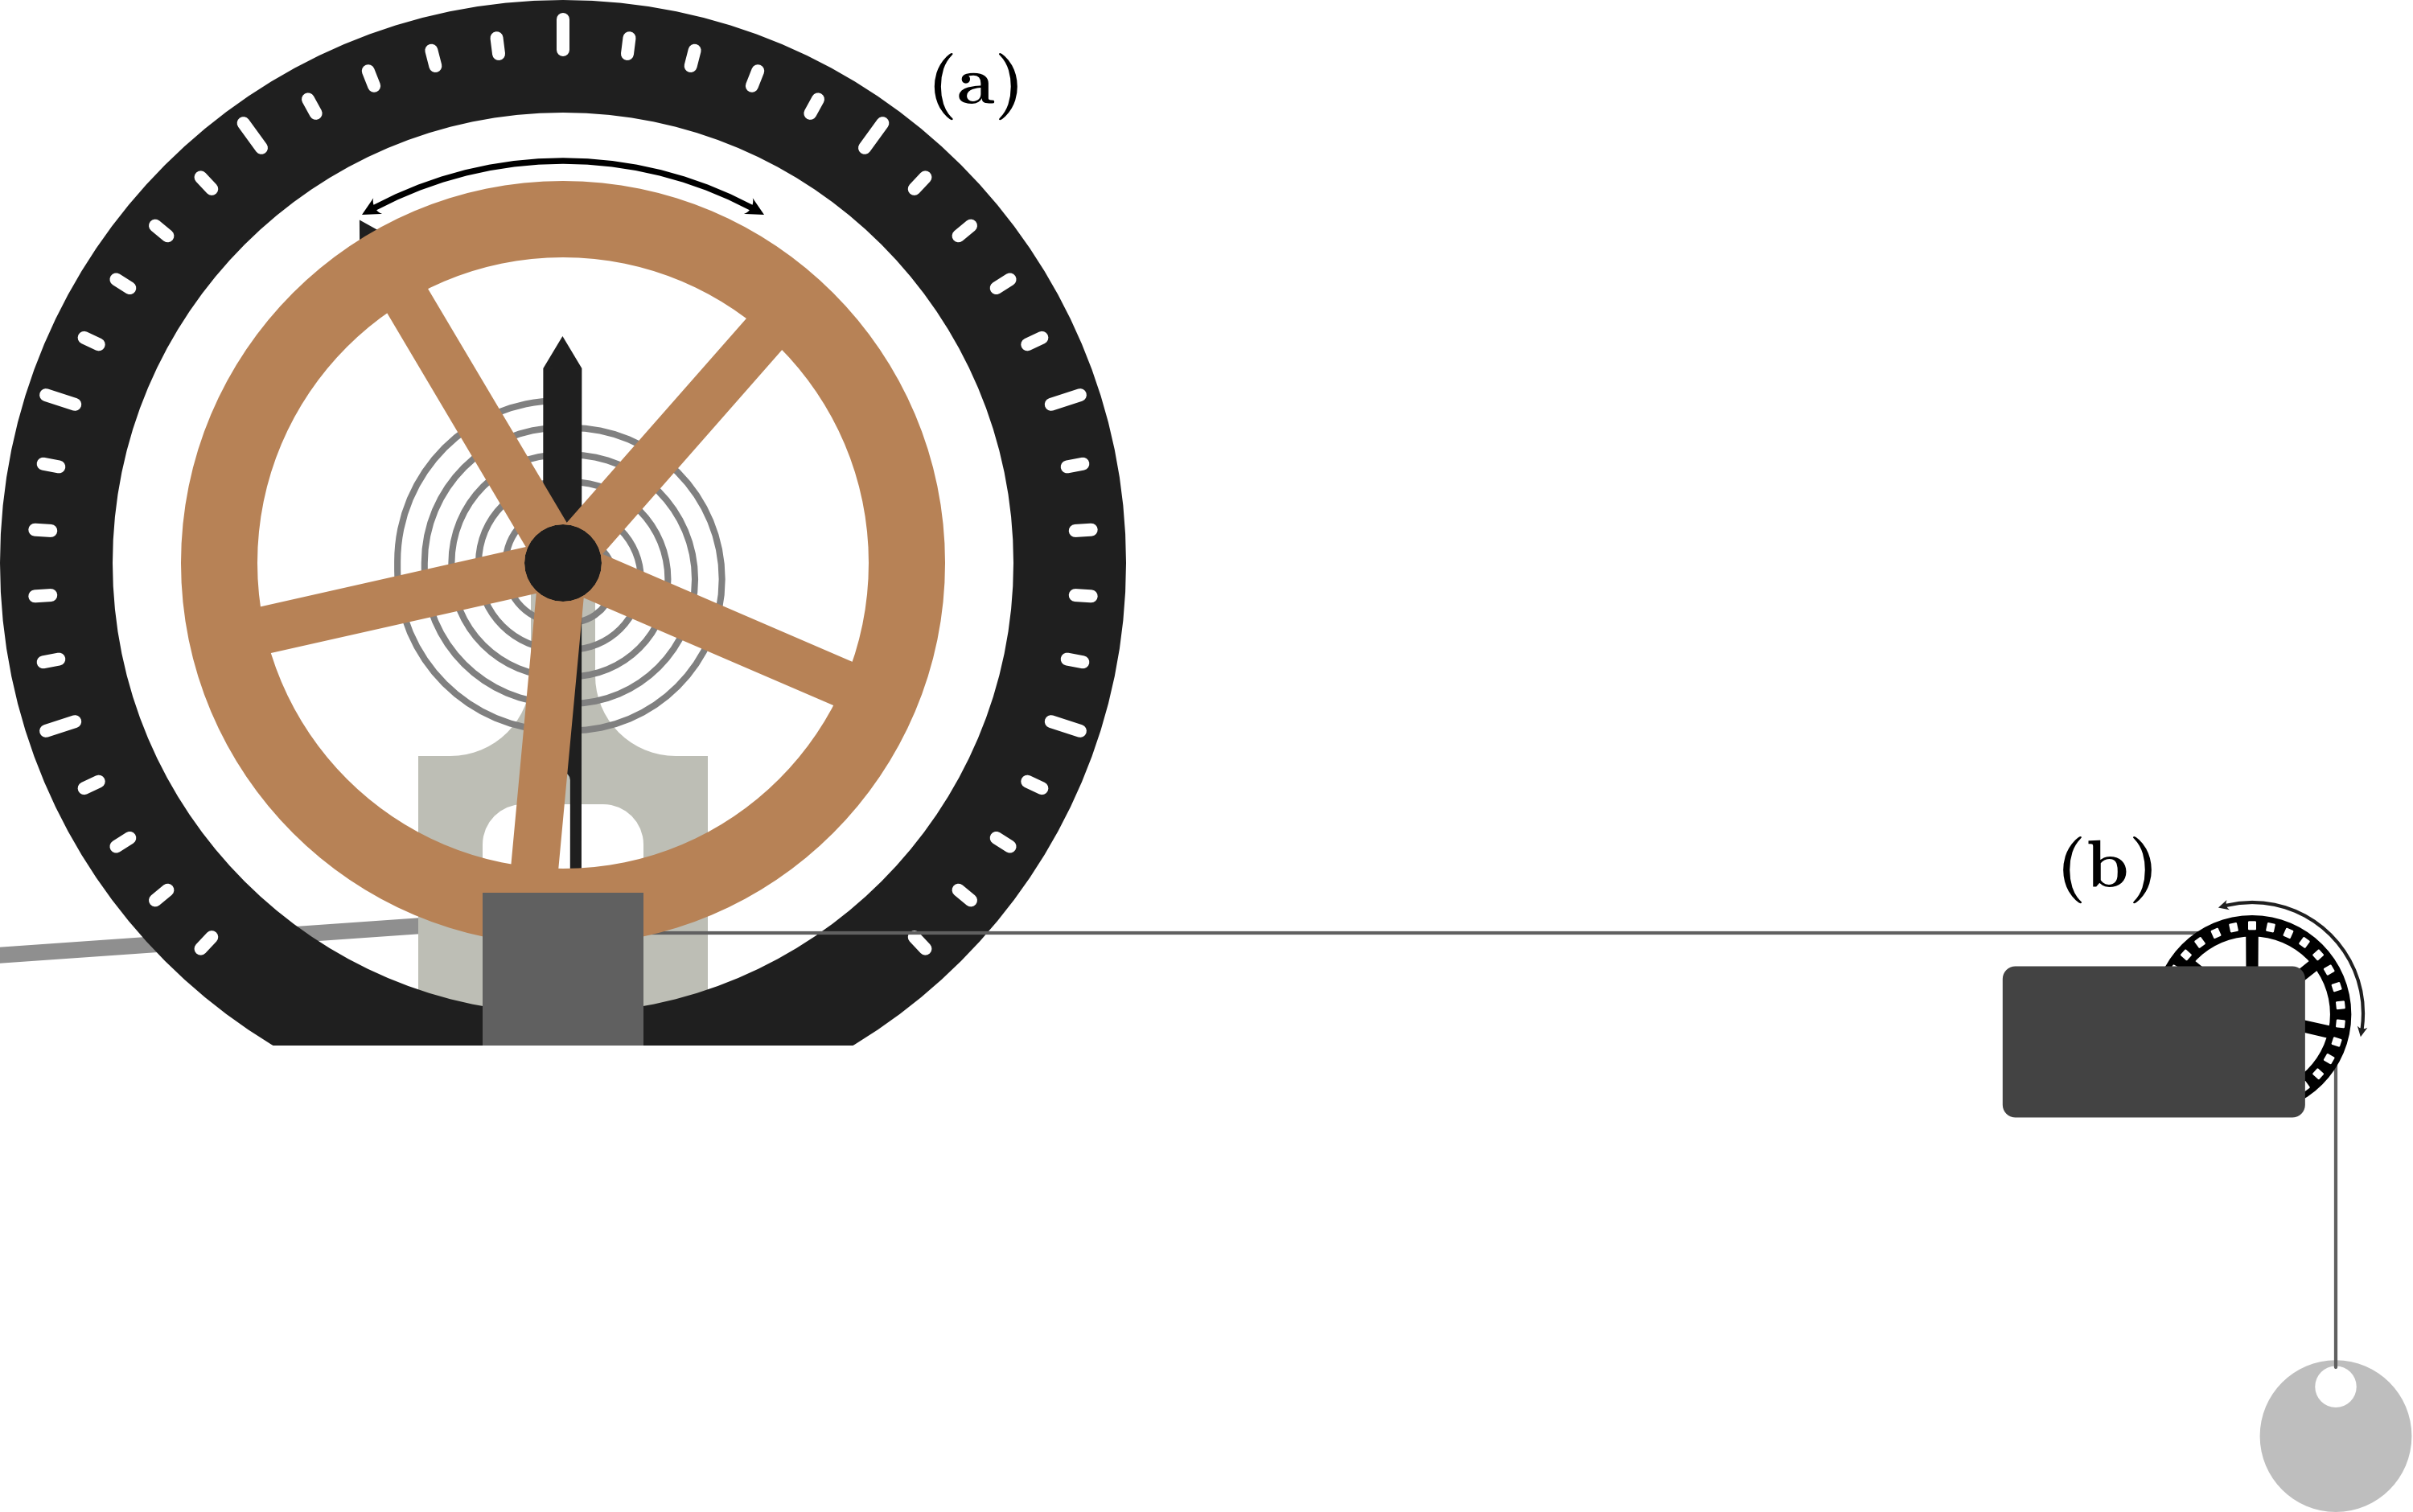
\includegraphics[width=\linewidth]{res/POHLFORZADO2.png}
	\captionof{figure}{Montaje experimental del péndulo de Pohl.
		\textbf{(a)} Péndulo de Pohl con una cuerda ligera sujetada al disco de cobre.
		La cuerda está amarrada a un anillo liviano para tensarla.
		\textbf{(b)} Polea ligera sosteniendo la cuerda. El sensor detecta la rotación
		de la polea permitiendo registrar la amplitud con respecto al tiempo.
	}
	\label{fig:montaje}
\end{figure}

\subsection*{3. Procedimiento}
En la practica experimental se dejó oscilar el péndulo de Pohl cinco veces, una sin
amortiguamiento y cuatro con amortiguamiento variable, manteniendo la amplitud angular
inicial constante en $\approx\qty{36}{\degree}$. Para cada valor de amortiguamiento, se
forzó el péndulo con el motor, empleando la frecuencia de resonancia correspondiente.

Para empezar, en ambos extremos de la cuerda delgada, se ató el anillo ligero y el
disco de cobre del péndulo. Después, la cuerda se colocó sobre la polea ligera sin fricción
como se muestra en la Fig. (\ref{fig:montaje}). Para la primera serie de oscilaciones, se
dejó oscilar el péndulo libremente hasta que la resistencia propia del montaje lo detuviera.
Para las series de oscilaciones subsecuentes, utilizando la fuente de poder y el multímetro,
se suministraron corrientes de \qtylist{0,2;0,4;0,6;0,8}{\ampere} al electroimán, amortiguando
el sistema. 

Posteriormente, para realizar las oscilaciones forzadas, se colocó el péndulo en su posición de
equilibrio y se suministraron voltajes de \qtylist{7,30;7,13;7,05;6,95}{\volt} al motor,
con cada valor correspondiendo a las corrientes de amortiguamiento empleadas en el proceso
anterior. Se dejó estabilizar cada serie de oscilaciones forzadas antes de registrar la
amplitud máxima.

Finalmente, además del voltaje suministrado al motor para el amortiguamiento
con corriente de \qty{0,4}{\ampere}, se suministraron voltajes entre 3...\qty{12}{\volt}, con
incrementos de \qty{1}{\volt}, en una serie de oscilaciones distinta. El registro de datos se
realizó mediante el programa \textit{CASSY Lab 2}.